\documentclass[aspectratio=43]{beamer}

%%%%%% 导入包 %%%%%%
\usepackage{xeCJK}
\usepackage{graphicx}
\usepackage{xcolor}
\usepackage{cite}
\usepackage{indentfirst}
\usepackage{amsmath}
\usepackage{amssymb}
\usepackage{times}

\usepackage{ctex}
\usepackage{geometry}
\usepackage{graphicx}
\usepackage{multirow}
\usepackage{array}
\usepackage{float}

\usepackage[super,square,comma,sort&compress]{natbib}
\usepackage{listings}
\usepackage{xcolor}
\colorlet{punct}{red!60!black}
\definecolor{background}{HTML}{EEEEEE}
\definecolor{delim}{RGB}{20,105,176}
\colorlet{numb}{magenta!60!black}

\lstdefinelanguage{json}{
    basicstyle=\ttfamily\scriptsize,
    numbers=left,
    numberstyle=\ttfamily\scriptsize,
    stepnumber=1,
    numbersep=4pt,
    showstringspaces=false,
    breaklines=true,
    frame=lines,
    % backgroundcolor=\color{background},
    literate=
     *{0}{{{\color{numb}0}}}{1}
      {1}{{{\color{numb}1}}}{1}
      {2}{{{\color{numb}2}}}{1}
      {3}{{{\color{numb}3}}}{1}
      {4}{{{\color{numb}4}}}{1}
      {5}{{{\color{numb}5}}}{1}
      {6}{{{\color{numb}6}}}{1}
      {7}{{{\color{numb}7}}}{1}
      {8}{{{\color{numb}8}}}{1}
      {9}{{{\color{numb}9}}}{1}
      {:}{{{\color{punct}{:}}}}{1}
      {,}{{{\color{punct}{,}}}}{1}
      {\{}{{{\color{delim}{\{}}}}{1}
      {\}}{{{\color{delim}{\}}}}}{1}
      {[}{{{\color{delim}{[}}}}{1}
      {]}{{{\color{delim}{]}}}}{1},
}


\lstset{
    columns=flexible,
    tabsize = 4,
    basicstyle=\ttfamily\scriptsize,                     % 字体大小
    backgroundcolor=\color{white},                       % 背景颜色
    numbers=left,                                        % 在左侧显示行号
    keywordstyle=\color[RGB]{40,40,255},                 % 设定关键字颜色
    % frame=trbl,
    stepnumber=1,
    numbersep=4pt,
    breaklines=true,
    frame=lines,
    numberstyle=\ttfamily\scriptsize\color{darkgray},    % 设定行号格式
    commentstyle=\it\color[RGB]{0,96,96},                % 设置代码注释的格式
    stringstyle=\rmfamily\slshape\color[RGB]{128,0,0},   % 设置字符串格式
    showstringspaces=false,                              % 不显示字符串中的空格
    language=python,                                     % 设置语言
}
\mode<presentation>
{
  \usetheme{CambridgeUS}
  \usecolortheme{beaver}
  \usefonttheme{default}      % or try serif, structurebold, ...
  \setbeamertemplate{navigation symbols}{}
  \setbeamertemplate{caption}[numbered]
}

\usepackage[english]{babel}
\usepackage[utf8x]{inputenc}
\usepackage{graphicx}
\usepackage{ulem}

\setbeamertemplate{itemize items}{\color{black}$\bullet$}
\graphicspath{{figure/}}

\defbeamertemplate{subsection in toc}{bullets}{%
  \leavevmode
  \parbox[t]{1em}{\textbullet\hfill}%
  \parbox[t]{\dimexpr\textwidth-1em\relax}{\inserttocsubsection}\par}

\defbeamertemplate{section in toc}{sections numbered roman}{%
  \leavevmode%
  \MakeUppercase{\romannumeral\inserttocsectionnumber}.\ %
  \inserttocsection\par}

\setbeamertemplate{section in toc}[sections numbered roman]
\setbeamertemplate{subsection in toc}[bullets]

%%%%%%%%%%%%%%%%%%%%%%%%%%%%%%%%%%%%%%%%%%%%%%%%%%%%%%%%%%%%%%%%%%%%%%%%%%%%%%%%%%
%%%%%%%%%%%%%                       Title                         %%%%%%%%%%%%%%%%
%%%%%%%%%%%%%%%%%%%%%%%%%%%%%%%%%%%%%%%%%%%%%%%%%%%%%%%%%%%%%%%%%%%%%%%%%%%%%%%%%%
\title{机器学习回顾 \& Location实验}
\author{游浩然 }
\institute[\bf HUST]{u201515429@hust.edu.cn}
\medskip
\date{\today}

\begin{document}

\begin{frame}
  \titlepage
\end{frame}

%%%%%%%%%%%%%%%%%%%%%%%%%%%%%%%%%%%%%%%%%%%%%%%%%%%%%%%%%%%%%%%%%%%%%%%%%%%%%%%%%%
%%%%%%%%%%%%%                       Content                       %%%%%%%%%%%%%%%%
%%%%%%%%%%%%%%%%%%%%%%%%%%%%%%%%%%%%%%%%%%%%%%%%%%%%%%%%%%%%%%%%%%%%%%%%%%%%%%%%%%

\AtBeginSection[]
{
\begin{frame}<beamer>{Table of Contents}
\tableofcontents[currentsection,currentsubsection,
    hideothersubsections,
    sectionstyle=show/shaded,
]
\end{frame}
}

%%%%%%%%%%%%%%%%%%%%%%%%%%%%%%%%%%%%%%%%%%%%%%%%%%%%%%%%%%%%%%%%%%%%%%%%%%%%%%%%%%
%%%%%%%%%%%%%                       Section                       %%%%%%%%%%%%%%%%
%%%%%%%%%%%%%%%%%%%%%%%%%%%%%%%%%%%%%%%%%%%%%%%%%%%%%%%%%%%%%%%%%%%%%%%%%%%%%%%%%%

\section{机器学习回顾}
% frame 1
\begin{frame}{机器学习}
\begin{itemize}
  \item 传统机器学习
  \begin{itemize}
    \item 优化问题
    \item 分/聚类问题
    \item 预测问题
  \end{itemize}
  \item 深度学习
  \begin{figure}[!htbp]
    \centering
    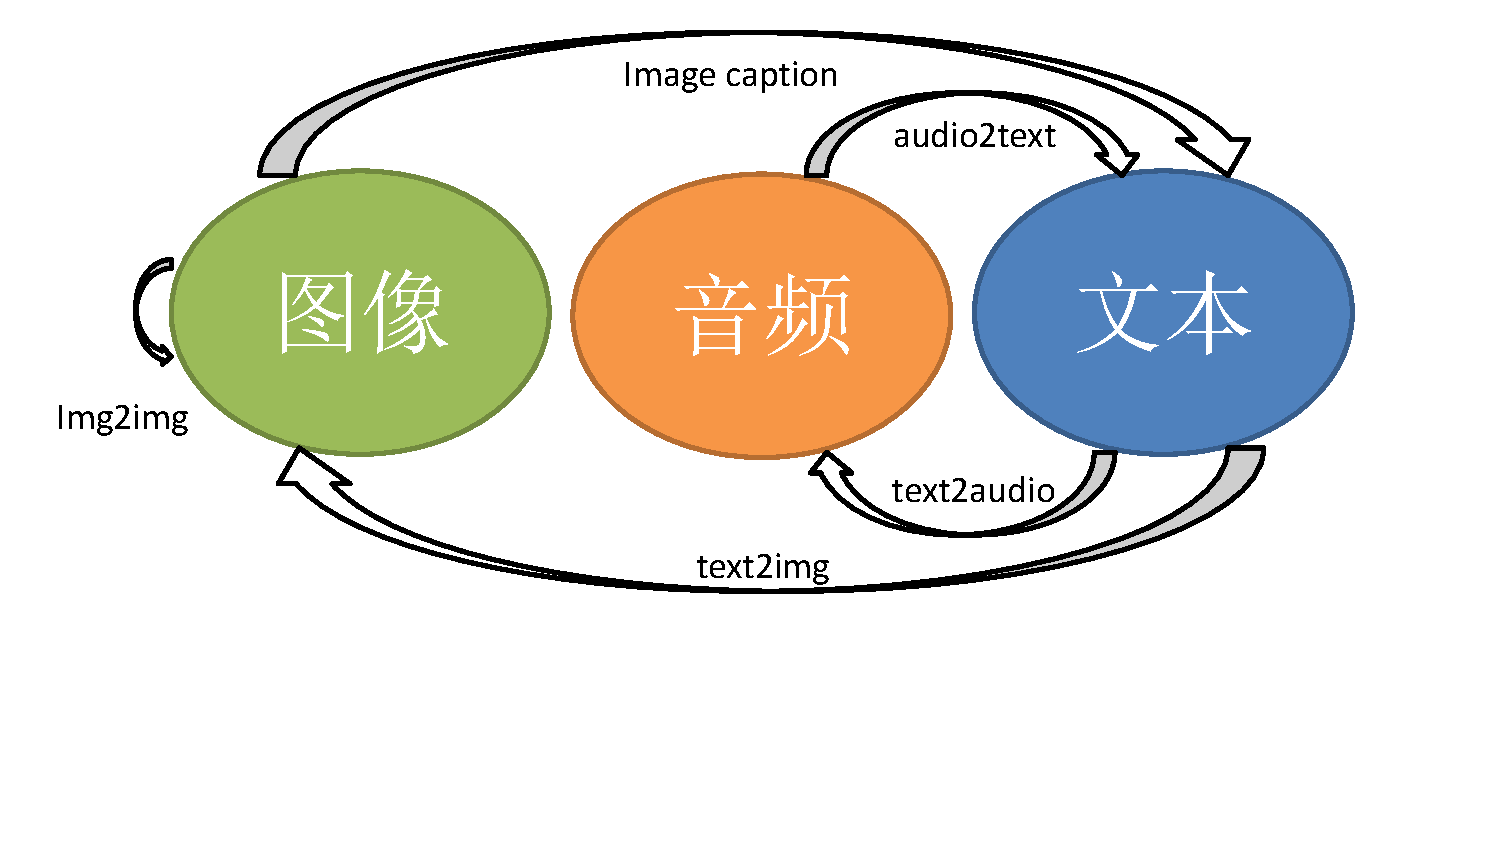
\includegraphics[width=8cm]{dl.pdf}
  \end{figure}
\end{itemize}
\end{frame}

\subsection{优化问题}
\begin{frame}{优化问题}
\begin{block}{Example: EV Charger Location for Ireland (ICM 2018)}
\end{block}
\begin{itemize}
  \item destination charging designed for charging for several hours at a time or even overnight.
  \item supercharging designed for longer road trips to provide up to 170 miles of range in as little as 30 minutes of charging.
\end{itemize}
one of five tasks:
\begin{itemize}
  \item Determine the optimal number, placement and distribution of charging stations if your country could migrate all their personal passengers vehicles to all-electric vehicles instantaneously.
  \item Present a proposal for evolving the charging network of your chosen country from zero chargers to a full electric-vehicle system.
  \item Based on your growth plan, what is the timeline you propose for the full evolution to electric vehicles in your chosen country.
\end{itemize}
\end{frame}

\subsection{分/聚类问题}
\begin{frame}{分/聚类问题}
\begin{block}{Example: 对通讯记录进行社群划分 (华中赛 2017)}
\end{block}
\vspace{1cm}
\begin{itemize}
  \item 给定无向图,区分个体差异,实现分群
  \item 给定有向图,刻画任意两点间的相似关系
  \item 给出某营业部近三个月的内部通讯记录,结合并完善问题1,2的数学模型,实现个体的分群。
  \item 考虑通讯的位置,时间,通话频率等多种因素建立综合的数学模型,挖掘更多的信息。
\end{itemize}
\vspace{1cm}
\end{frame}

\subsection{预测问题}
\begin{frame}{预测问题}
\begin{block}{Example: 高炉炼铁-铁水含硅量预测 (MathorCup 2017)}
\end{block}
\vspace{0.3cm}
炼铁过程依时间序列采集的工艺参数是一个高维的时间序列,影响因素数以百计。其终极生产指标产量、能耗、铁水质量等指标都与炼铁过程中的一项控制性中间指标——炉温,即铁水含硅量[Si]密切相关。
\begin{itemize}
  \item 从给定数据表中[Si]-[S]-FL-PML依序号排列的1000炉生产数据中,自主选择学习样本和算法,建立[Si]预测动态数学模型,包括一步预测和两步预测。
  \item 自主选择验证样本,验证预测成功率,包括数值预测成功率和炉温升降方向预测成功率,并讨论其动态预测控制的可行性。
  \item 建立质量指标[S]的优化数学模型,讨论按照优化模型计算结果进行[Si]预测控制的预期效果。
\end{itemize}
\end{frame}

%%%%%%%%%%%%%%%%

\section{Location Assignment}
\subsection{Method}
\begin{frame}{KNN}
main-idea:
\begin{itemize}
  \item 用K个最近邻样本输出的平均值作为回归预测值。
\end{itemize}
\vspace{1cm}
feature selection:
\begin{itemize}
  \item 取训练集和测试集feature的交集,总特征数为423
  \item 将信号强度0变为极弱信号强度-100
  \item 按比例划分训练集和交叉验证集。
\end{itemize}
\end{frame}

\subsection{Result}
\begin{frame}{Distribution}
\begin{figure}[!htbp]
  \centering
  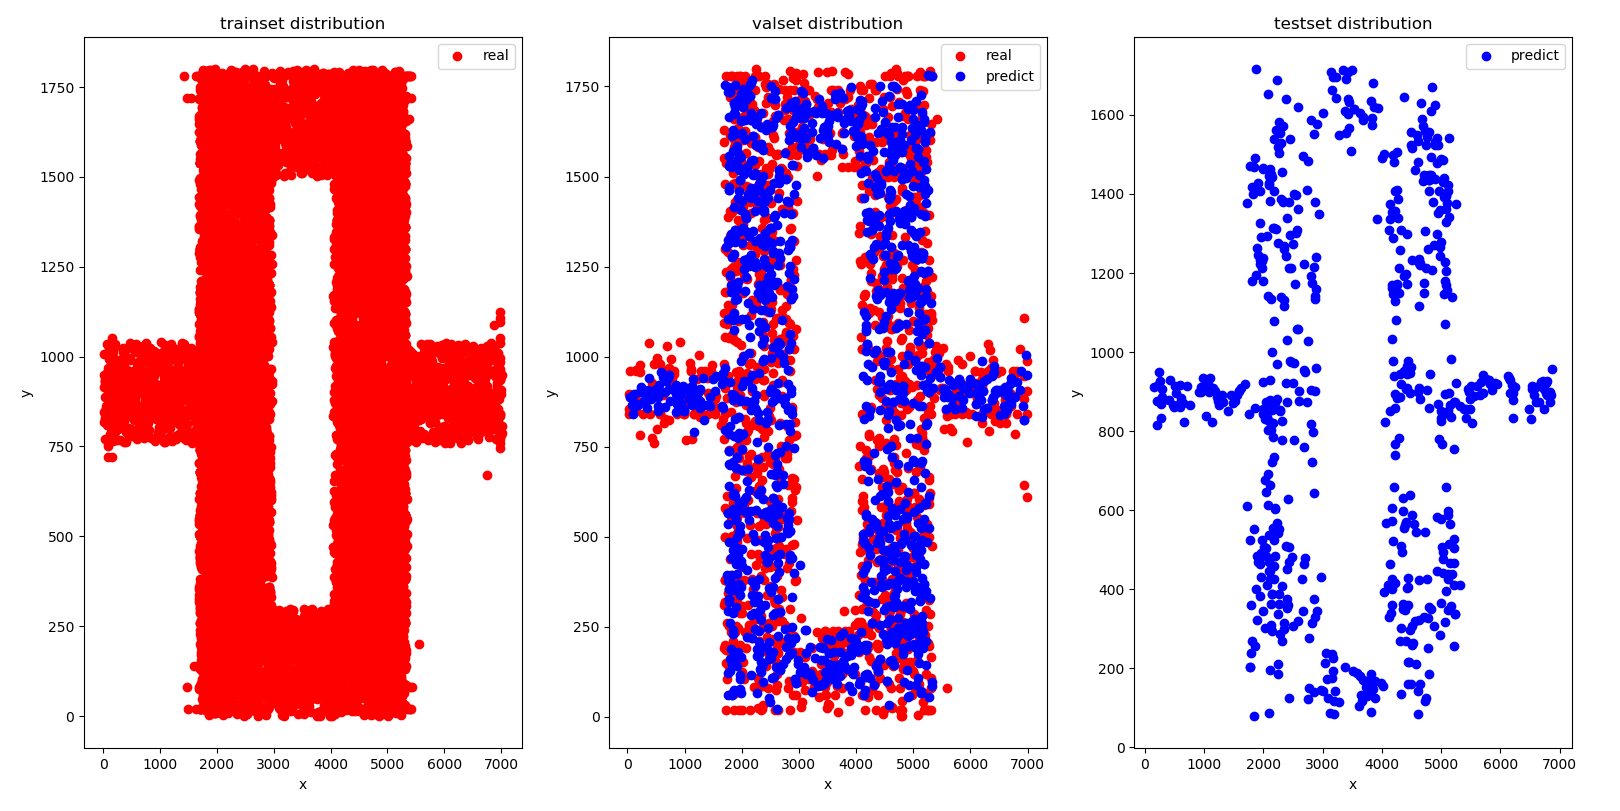
\includegraphics[width=12cm]{distribution.png}
  \caption{Distribution}
\end{figure}
\end{frame}

\begin{frame}{CDF}
\begin{figure}
  \centering
  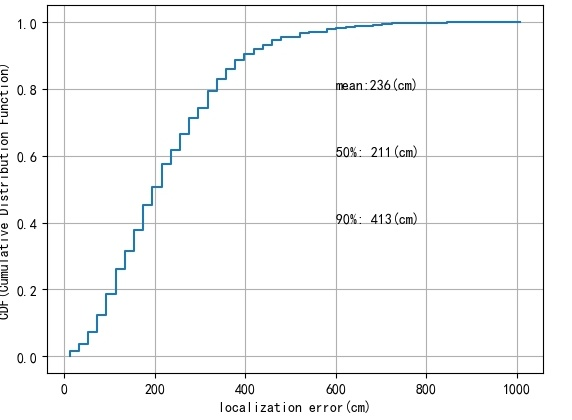
\includegraphics[width=8cm]{cdf.png}
  \caption{Cumulative Distribution Function}
\end{figure}
\end{frame}

\begin{frame}
\begin{block}{Thank You.}
\end{block}
\end{frame}

\end{document}
